\documentclass[border=5pt]{standalone}
\usepackage[utf8]{inputenc}
\usepackage{amssymb}
\usepackage{amsmath}
\usepackage{tikz}
\usetikzlibrary{arrows.meta}

\begin{document}
\nopagecolor
\begin{tabular}{l | l}
    \textbf{Undirected Graph} (From Held and Karp paper) & \textbf{Directed Graph} (From my program) \\
    \hline
    Iteration 1: \\
    Starting configuration: $(\emptyset, \emptyset, \begin{bmatrix} 0 & 0 & 0 & 0 & 0 & 0 \end{bmatrix}, 196)$ 
    &
    Starting configuration: $(\emptyset, \emptyset, \begin{bmatrix}
        0 & 0 & 0 & 0 & 0 & 0
    \end{bmatrix}, 196)$ \\
    Minimum 1-Trees: & Minimum 1-Arborescences: \\
    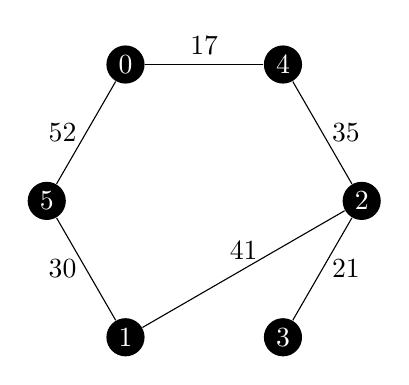
\begin{tikzpicture}
        \node[circle, inner sep=2pt, fill] (0) at (-1, 1.732) {\color{white} 0};
        \node[circle, inner sep=2pt, fill] (4) at (1, 1.732) {\color{white} 4};
        \node[circle, inner sep=2pt, fill] (2) at (2, 0) {\color{white} 2};
        \node[circle, inner sep=2pt, fill] (3) at (1, -1.732) {\color{white} 3};
        \node[circle, inner sep=2pt, fill] (1) at (-1, -1.732) {\color{white} 1};
        \node[circle, inner sep=2pt, fill] (5) at (-2, 0) {\color{white} 5};
        
        \draw (0) edge node[above]{17} (4);
        \draw (0) edge node[left]{52} (5);
        \draw (4) edge[right] node{35} (2);
        \draw (2) edge[above] node{41} (1);
        \draw (2) edge[right] node{21} (3);
        \draw (1) edge[left] node{30} (5);
    \end{tikzpicture}
    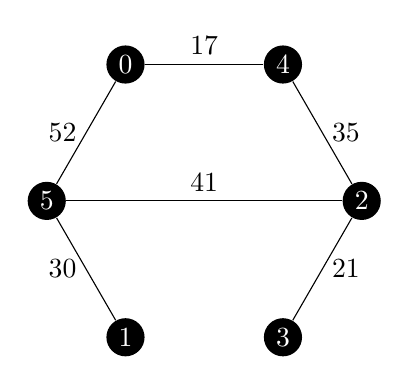
\begin{tikzpicture}
        \node[circle, inner sep=2pt, fill] (0) at (-1, 1.732) {\color{white} 0};
        \node[circle, inner sep=2pt, fill] (4) at (1, 1.732) {\color{white} 4};
        \node[circle, inner sep=2pt, fill] (2) at (2, 0) {\color{white} 2};
        \node[circle, inner sep=2pt, fill] (3) at (1, -1.732) {\color{white} 3};
        \node[circle, inner sep=2pt, fill] (1) at (-1, -1.732) {\color{white} 1};
        \node[circle, inner sep=2pt, fill] (5) at (-2, 0) {\color{white} 5};
        
        \draw (0) edge node[above]{17} (4);
        \draw (0) edge node[left]{52} (5);
        \draw (4) edge[right] node{35} (2);
        \draw (2) edge[above] node{41} (5);
        \draw (2) edge[right] node{21} (3);
        \draw (1) edge[left] node{30} (5);
    \end{tikzpicture}
    &
    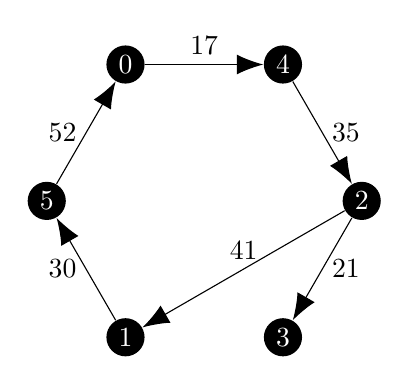
\begin{tikzpicture}
        \node[circle, inner sep=2pt, fill] (0) at (-1, 1.732) {\color{white} 0};
        \node[circle, inner sep=2pt, fill] (4) at (1, 1.732) {\color{white} 4};
        \node[circle, inner sep=2pt, fill] (2) at (2, 0) {\color{white} 2};
        \node[circle, inner sep=2pt, fill] (3) at (1, -1.732) {\color{white} 3};
        \node[circle, inner sep=2pt, fill] (1) at (-1, -1.732) {\color{white} 1};
        \node[circle, inner sep=2pt, fill] (5) at (-2, 0) {\color{white} 5};
        
        \draw[-{Latex[scale=2]}] (0) edge[above] node{17} (4);
        \draw[-{Latex[scale=2]}] (5) edge[left] node{52} (0);
        \draw[-{Latex[scale=2]}] (4) edge[right] node{35} (2);
        \draw[-{Latex[scale=2]}] (2) edge[above] node{41} (1);
        \draw[-{Latex[scale=2]}] (2) edge[right] node{21} (3);
        \draw[-{Latex[scale=2]}] (1) edge[left] node{30} (5);
    \end{tikzpicture}
    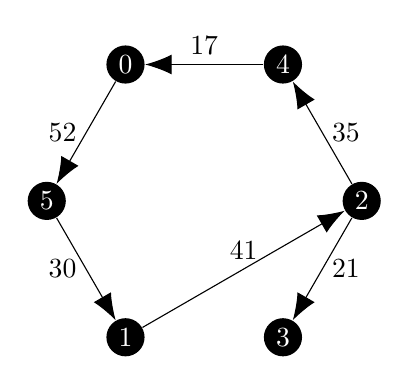
\begin{tikzpicture}
        \node[circle, inner sep=2pt, fill] (0) at (-1, 1.732) {\color{white} 0};
        \node[circle, inner sep=2pt, fill] (4) at (1, 1.732) {\color{white} 4};
        \node[circle, inner sep=2pt, fill] (2) at (2, 0) {\color{white} 2};
        \node[circle, inner sep=2pt, fill] (3) at (1, -1.732) {\color{white} 3};
        \node[circle, inner sep=2pt, fill] (1) at (-1, -1.732) {\color{white} 1};
        \node[circle, inner sep=2pt, fill] (5) at (-2, 0) {\color{white} 5};
        
        \draw[{Latex[scale=2]}-] (0) edge[above] node{17} (4);
        \draw[{Latex[scale=2]}-] (5) edge[left] node{52} (0);
        \draw[{Latex[scale=2]}-] (4) edge[right] node{35} (2);
        \draw[{Latex[scale=2]}-] (2) edge[above] node{41} (1);
        \draw[-{Latex[scale=2]}] (2) edge[right] node{21} (3);
        \draw[{Latex[scale=2]}-] (1) edge[left] node{30} (5);
    \end{tikzpicture}
    \\ &
    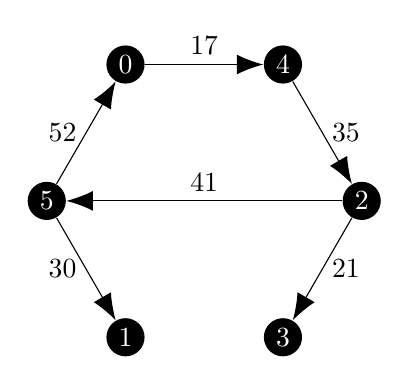
\begin{tikzpicture}
        \node[circle, inner sep=2pt, fill] (0) at (-1, 1.732) {\color{white} 0};
        \node[circle, inner sep=2pt, fill] (4) at (1, 1.732) {\color{white} 4};
        \node[circle, inner sep=2pt, fill] (2) at (2, 0) {\color{white} 2};
        \node[circle, inner sep=2pt, fill] (3) at (1, -1.732) {\color{white} 3};
        \node[circle, inner sep=2pt, fill] (1) at (-1, -1.732) {\color{white} 1};
        \node[circle, inner sep=2pt, fill] (5) at (-2, 0) {\color{white} 5};
        
        \draw[-{Latex[scale=2]}] (0) edge[above] node{17} (4);
        \draw[-{Latex[scale=2]}] (5) edge[left] node{52} (0);
        \draw[-{Latex[scale=2]}] (4) edge[right] node{35} (2);
        \draw[-{Latex[scale=2]}] (2) edge[above] node{41} (5);
        \draw[-{Latex[scale=2]}] (2) edge[right] node{21} (3);
        \draw[{Latex[scale=2]}-] (1) edge[left] node{30} (5);
    \end{tikzpicture}
    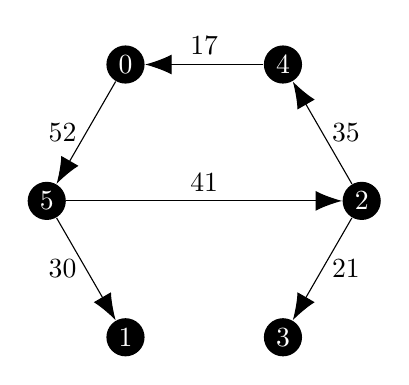
\begin{tikzpicture}
        \node[circle, inner sep=2pt, fill] (0) at (-1, 1.732) {\color{white} 0};
        \node[circle, inner sep=2pt, fill] (4) at (1, 1.732) {\color{white} 4};
        \node[circle, inner sep=2pt, fill] (2) at (2, 0) {\color{white} 2};
        \node[circle, inner sep=2pt, fill] (3) at (1, -1.732) {\color{white} 3};
        \node[circle, inner sep=2pt, fill] (1) at (-1, -1.732) {\color{white} 1};
        \node[circle, inner sep=2pt, fill] (5) at (-2, 0) {\color{white} 5};
        
        \draw[{Latex[scale=2]}-] (0) edge[above] node{17} (4);
        \draw[{Latex[scale=2]}-] (5) edge[left] node{52} (0);
        \draw[{Latex[scale=2]}-] (4) edge[right] node{35} (2);
        \draw[{Latex[scale=2]}-] (2) edge[above] node{41} (5);
        \draw[-{Latex[scale=2]}] (2) edge[right] node{21} (3);
        \draw[{Latex[scale=2]}-] (1) edge[left] node{30} (5);
    \end{tikzpicture}
    \\
    Vertex 3 out-of-kilter LOW & Vertex 3 out-of-kilter LOW \\
    $d = \begin{bmatrix} 0 & 0 & 0 & -1 & 0 & 0 \end{bmatrix}$ & $d = \begin{bmatrix} 0 & 0 & 0 & -1 & 0 & 0 \end{bmatrix}$ \\
    $\epsilon(\pi, d) = 5$ & $\epsilon(\pi, d) = 5$ \\
    New configuration: $(\emptyset, \emptyset, \begin{bmatrix} 0 & 0 & 0 & -5 & 0 & 0 \end{bmatrix}, 201)$ & New configuration: $(\emptyset, \emptyset, \begin{bmatrix} 0 & 0 & 0 & -5 & 0 & 0 \end{bmatrix}, 212)$ \\ \\
    Iteration 2: \\
    Minimum 1-Trees: & Minimum 1-Arborescences \\
    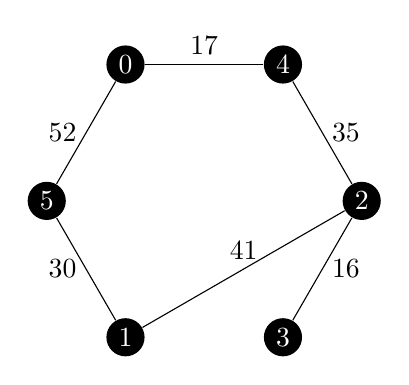
\begin{tikzpicture}
        \node[circle, inner sep=2pt, fill] (0) at (-1, 1.732) {\color{white} 0};
        \node[circle, inner sep=2pt, fill] (4) at (1, 1.732) {\color{white} 4};
        \node[circle, inner sep=2pt, fill] (2) at (2, 0) {\color{white} 2};
        \node[circle, inner sep=2pt, fill] (3) at (1, -1.732) {\color{white} 3};
        \node[circle, inner sep=2pt, fill] (1) at (-1, -1.732) {\color{white} 1};
        \node[circle, inner sep=2pt, fill] (5) at (-2, 0) {\color{white} 5};
        
        \draw (0) edge node[above]{17} (4);
        \draw (0) edge node[left]{52} (5);
        \draw (4) edge[right] node{35} (2);
        \draw (2) edge[above] node{41} (1);
        \draw (2) edge[right] node{16} (3);
        \draw (1) edge[left] node{30} (5);
    \end{tikzpicture}
    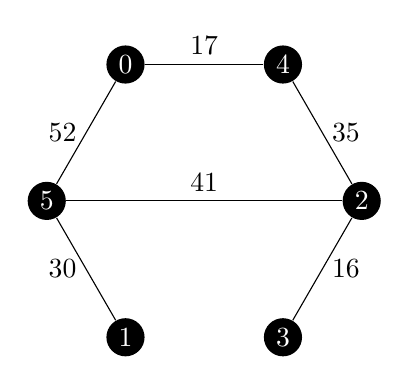
\begin{tikzpicture}
        \node[circle, inner sep=2pt, fill] (0) at (-1, 1.732) {\color{white} 0};
        \node[circle, inner sep=2pt, fill] (4) at (1, 1.732) {\color{white} 4};
        \node[circle, inner sep=2pt, fill] (2) at (2, 0) {\color{white} 2};
        \node[circle, inner sep=2pt, fill] (3) at (1, -1.732) {\color{white} 3};
        \node[circle, inner sep=2pt, fill] (1) at (-1, -1.732) {\color{white} 1};
        \node[circle, inner sep=2pt, fill] (5) at (-2, 0) {\color{white} 5};
        
        \draw (0) edge node[above]{17} (4);
        \draw (0) edge node[left]{52} (5);
        \draw (4) edge[right] node{35} (2);
        \draw (2) edge[above] node{41} (5);
        \draw (2) edge[right] node{16} (3);
        \draw (1) edge[left] node{30} (5);
    \end{tikzpicture}
    &
    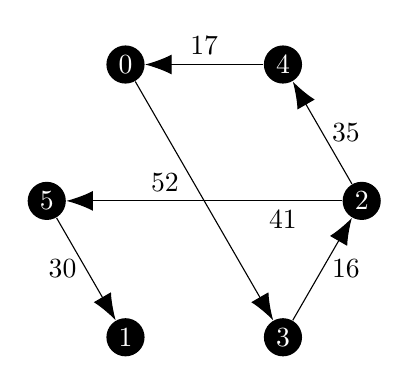
\begin{tikzpicture}
        \node[circle, inner sep=2pt, fill] (0) at (-1, 1.732) {\color{white} 0};
        \node[circle, inner sep=2pt, fill] (4) at (1, 1.732) {\color{white} 4};
        \node[circle, inner sep=2pt, fill] (2) at (2, 0) {\color{white} 2};
        \node[circle, inner sep=2pt, fill] (3) at (1, -1.732) {\color{white} 3};
        \node[circle, inner sep=2pt, fill] (1) at (-1, -1.732) {\color{white} 1};
        \node[circle, inner sep=2pt, fill] (5) at (-2, 0) {\color{white} 5};
        
        \draw[{Latex[scale=2]}-] (0) edge[above] node{17} (4);
        \draw[{Latex[scale=2]}-] (3) edge[left] node[xshift=-0.2cm, yshift=0.23cm]{52} (0);
        \draw[{Latex[scale=2]}-] (4) edge[right] node{35} (2);
        \draw[-{Latex[scale=2]}] (2) edge[below] node[xshift=1cm]{41} (5);
        \draw[{Latex[scale=2]}-] (2) edge[right] node{16} (3);
        \draw[{Latex[scale=2]}-] (1) edge[left] node{30} (5);
    \end{tikzpicture}
    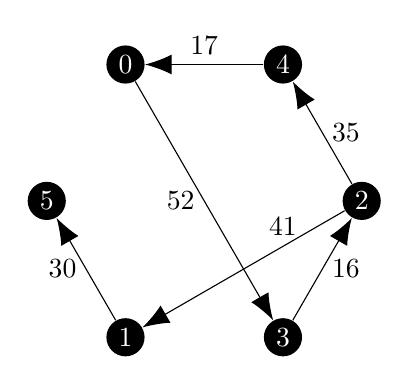
\begin{tikzpicture}
        \node[circle, inner sep=2pt, fill] (0) at (-1, 1.732) {\color{white} 0};
        \node[circle, inner sep=2pt, fill] (4) at (1, 1.732) {\color{white} 4};
        \node[circle, inner sep=2pt, fill] (2) at (2, 0) {\color{white} 2};
        \node[circle, inner sep=2pt, fill] (3) at (1, -1.732) {\color{white} 3};
        \node[circle, inner sep=2pt, fill] (1) at (-1, -1.732) {\color{white} 1};
        \node[circle, inner sep=2pt, fill] (5) at (-2, 0) {\color{white} 5};
        
        \draw[{Latex[scale=2]}-] (0) edge[above] node{17} (4);
        \draw[{Latex[scale=2]}-] (3) edge[left] node{52} (0);
        \draw[{Latex[scale=2]}-] (4) edge[right] node{35} (2);
        \draw[-{Latex[scale=2]}] (2) edge[above] node[xshift=0.5cm, yshift=0.3cm]{41} (1);
        \draw[{Latex[scale=2]}-] (2) edge[right] node{16} (3);
        \draw[-{Latex[scale=2]}] (1) edge[left] node{30} (5);
    \end{tikzpicture}
    \\
    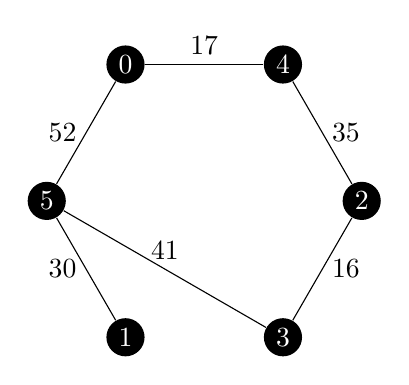
\begin{tikzpicture}
        \node[circle, inner sep=2pt, fill] (0) at (-1, 1.732) {\color{white} 0};
        \node[circle, inner sep=2pt, fill] (4) at (1, 1.732) {\color{white} 4};
        \node[circle, inner sep=2pt, fill] (2) at (2, 0) {\color{white} 2};
        \node[circle, inner sep=2pt, fill] (3) at (1, -1.732) {\color{white} 3};
        \node[circle, inner sep=2pt, fill] (1) at (-1, -1.732) {\color{white} 1};
        \node[circle, inner sep=2pt, fill] (5) at (-2, 0) {\color{white} 5};
        
        \draw (0) edge node[above]{17} (4);
        \draw (0) edge node[left]{52} (5);
        \draw (4) edge[right] node{35} (2);
        \draw (5) edge[above] node{41} (3);
        \draw (2) edge[right] node{16} (3);
        \draw (1) edge[left] node{30} (5);
    \end{tikzpicture}
    &
    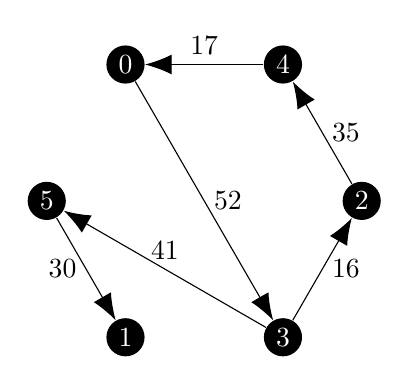
\begin{tikzpicture}
        \node[circle, inner sep=2pt, fill] (0) at (-1, 1.732) {\color{white} 0};
        \node[circle, inner sep=2pt, fill] (4) at (1, 1.732) {\color{white} 4};
        \node[circle, inner sep=2pt, fill] (2) at (2, 0) {\color{white} 2};
        \node[circle, inner sep=2pt, fill] (3) at (1, -1.732) {\color{white} 3};
        \node[circle, inner sep=2pt, fill] (1) at (-1, -1.732) {\color{white} 1};
        \node[circle, inner sep=2pt, fill] (5) at (-2, 0) {\color{white} 5};
        
        \draw[{Latex[scale=2]}-] (0) edge[above] node{17} (4);
        \draw[{Latex[scale=2]}-] (3) edge[right] node{52} (0);
        \draw[{Latex[scale=2]}-] (4) edge[right] node{35} (2);
        \draw[-{Latex[scale=2]}] (3) edge[above] node{41} (5);
        \draw[{Latex[scale=2]}-] (2) edge[right] node{16} (3);
        \draw[{Latex[scale=2]}-] (1) edge[left] node{30} (5);
    \end{tikzpicture}
    \\
\end{tabular}
\end{document}